
\chapter{Documentation Technique du Raspberry Pi B+}
\label{annexe:rpi}

\section{Définition}


\textit{\og Le Raspberry Pi est un nano-ordinateur monocarte à processeur ARM conçu par le créateur de jeux vidéo David Braben, dans le cadre de sa fondation Raspberry Pi.}

\textit{Cet ordinateur, qui a la taille d'une carte de crédit, est destiné à encourager l'apprentissage de la programmation informatique2 ; il permet l'exécution de plusieurs variantes du système d'exploitation libre GNU/Linux et des logiciels compatibles. Il est fourni nu (carte mère seule, sans boîtier, alimentation, clavier, souris ni écran) dans l'objectif de diminuer les coûts et de permettre l'utilisation de matériel de récupération.}

\textit{Son prix de vente était estimé à 25 \$, soit 19,09 \euro, début mai 2011. Les premiers exemplaires ont été mis en vente le 29 février 2012 pour environ 25 \euro. Début 2015, plus de cinq millions de Raspberry Pi ont été vendus. De multiples versions ont été développées (voir la liste ci-dessous), on trouve les dernières à un peu plus de 25 \euro~ pour le B+, à un peu plus de 30 \euro~ pour le Pi 2 (2015) et à un peu plus de 45 \euro~ pour le Pi 3 (2016)\fg{}} Wikipédia \cite{wiki_rpi}

\section{Caractéristique et connectiques}
\begin{tabular}[c]{|l|l|}
\hline
\multicolumn{2}{|c|}{Caractéristiques}\\
\hline
Micro-contrôleur &	Broadcom BCM2835 ARM1176JZFS\\
Vitesse d'horloge& 	700 MHz\\
RAM &	512 Mo\\
\hline
\multicolumn{2}{c}{}\\
\hline
\multicolumn{2}{|c|}{Connectiques}\\
\hline
Port(s) USB &	4\\
Port Ethernet / RJ45 &	1\\
Connecteur(s) audio analogique &	1 sortie jack 3,5 mm\\
HDMI 	&1\\
Port pour carte mémoire 	&1 port micro SD\\
Alimentation &	via port micro USB 5V\\
\hline
\end{tabular}

\newpage
\section{Schéma technique}



\begin{figure}[!h]
  \centering
  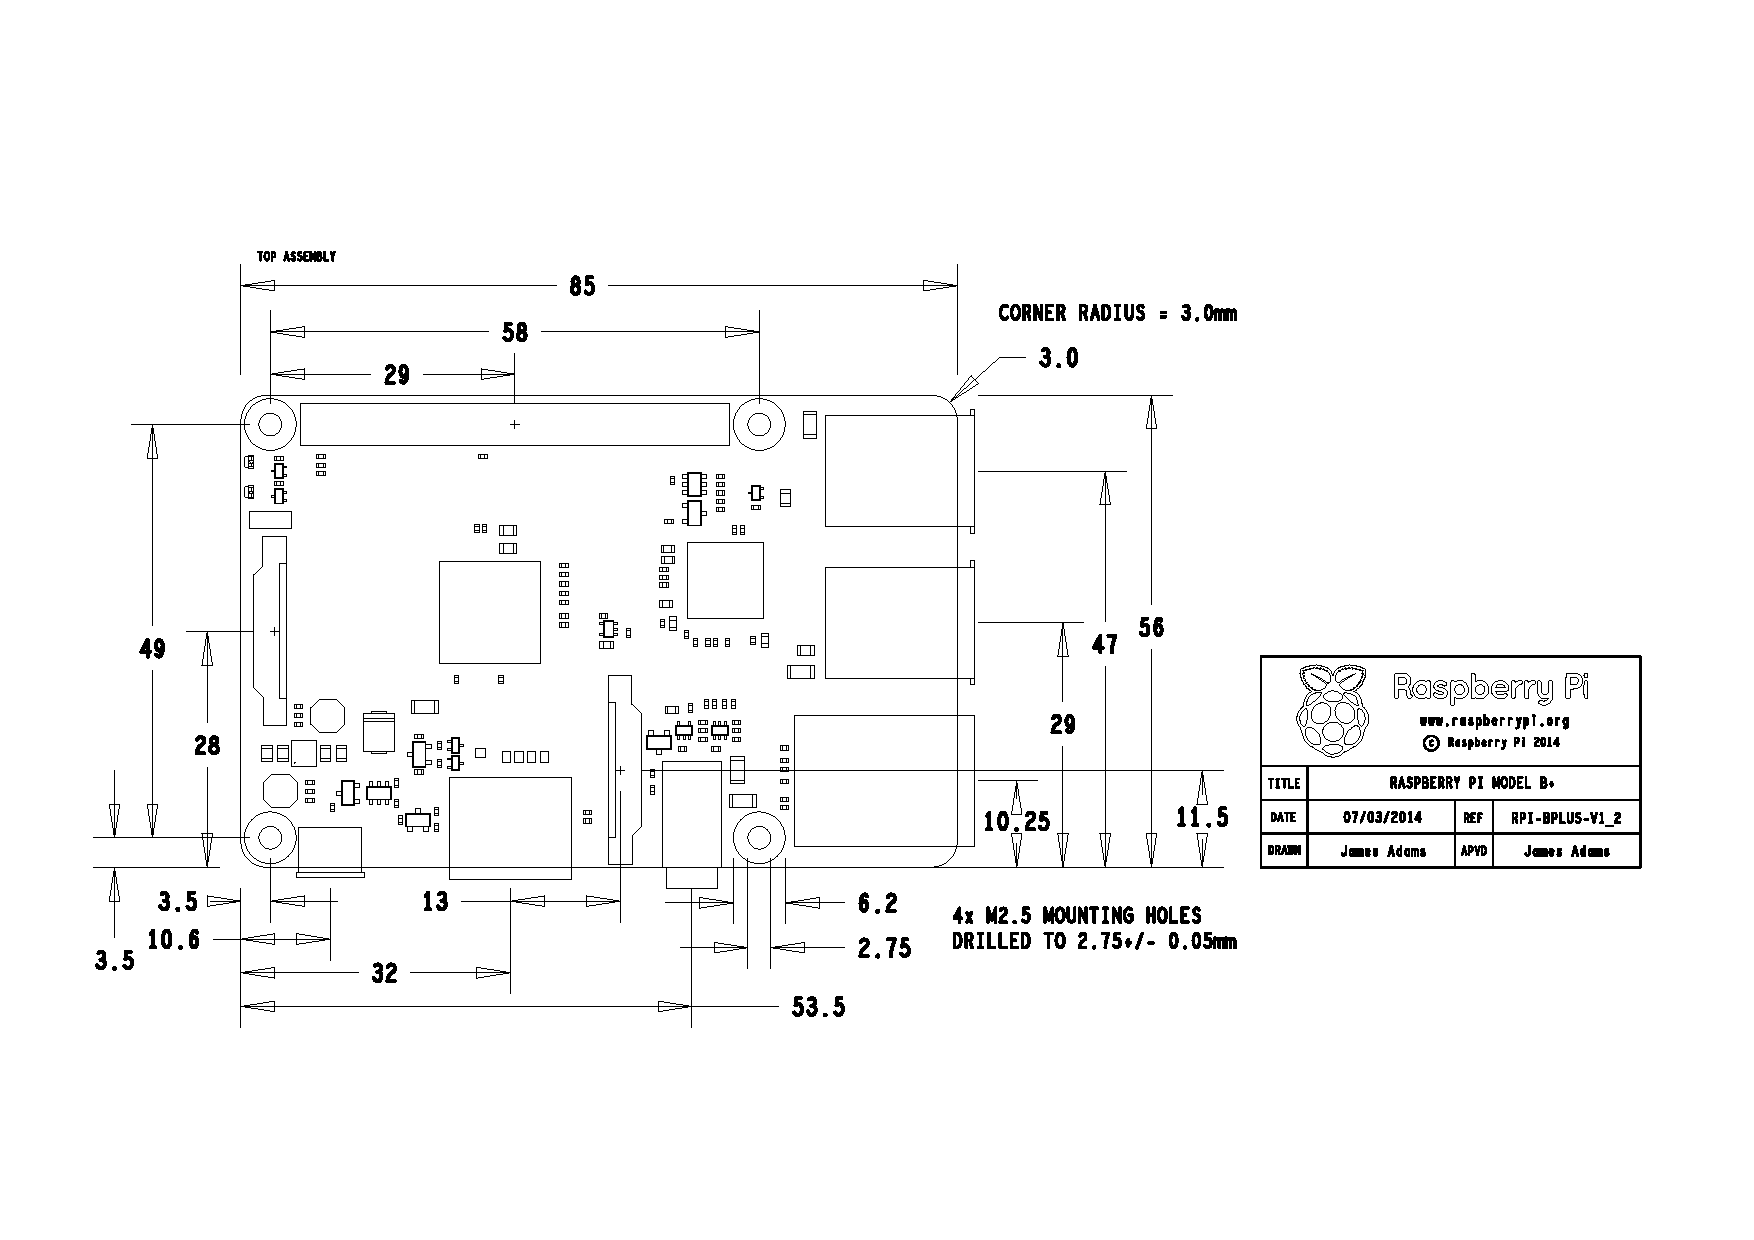
\includegraphics[width=\textwidth]{raspberrypi_doc_mecanique}
  \caption{Dessin mecanique}
\end{figure}

\begin{figure}[!h]
  \centering
  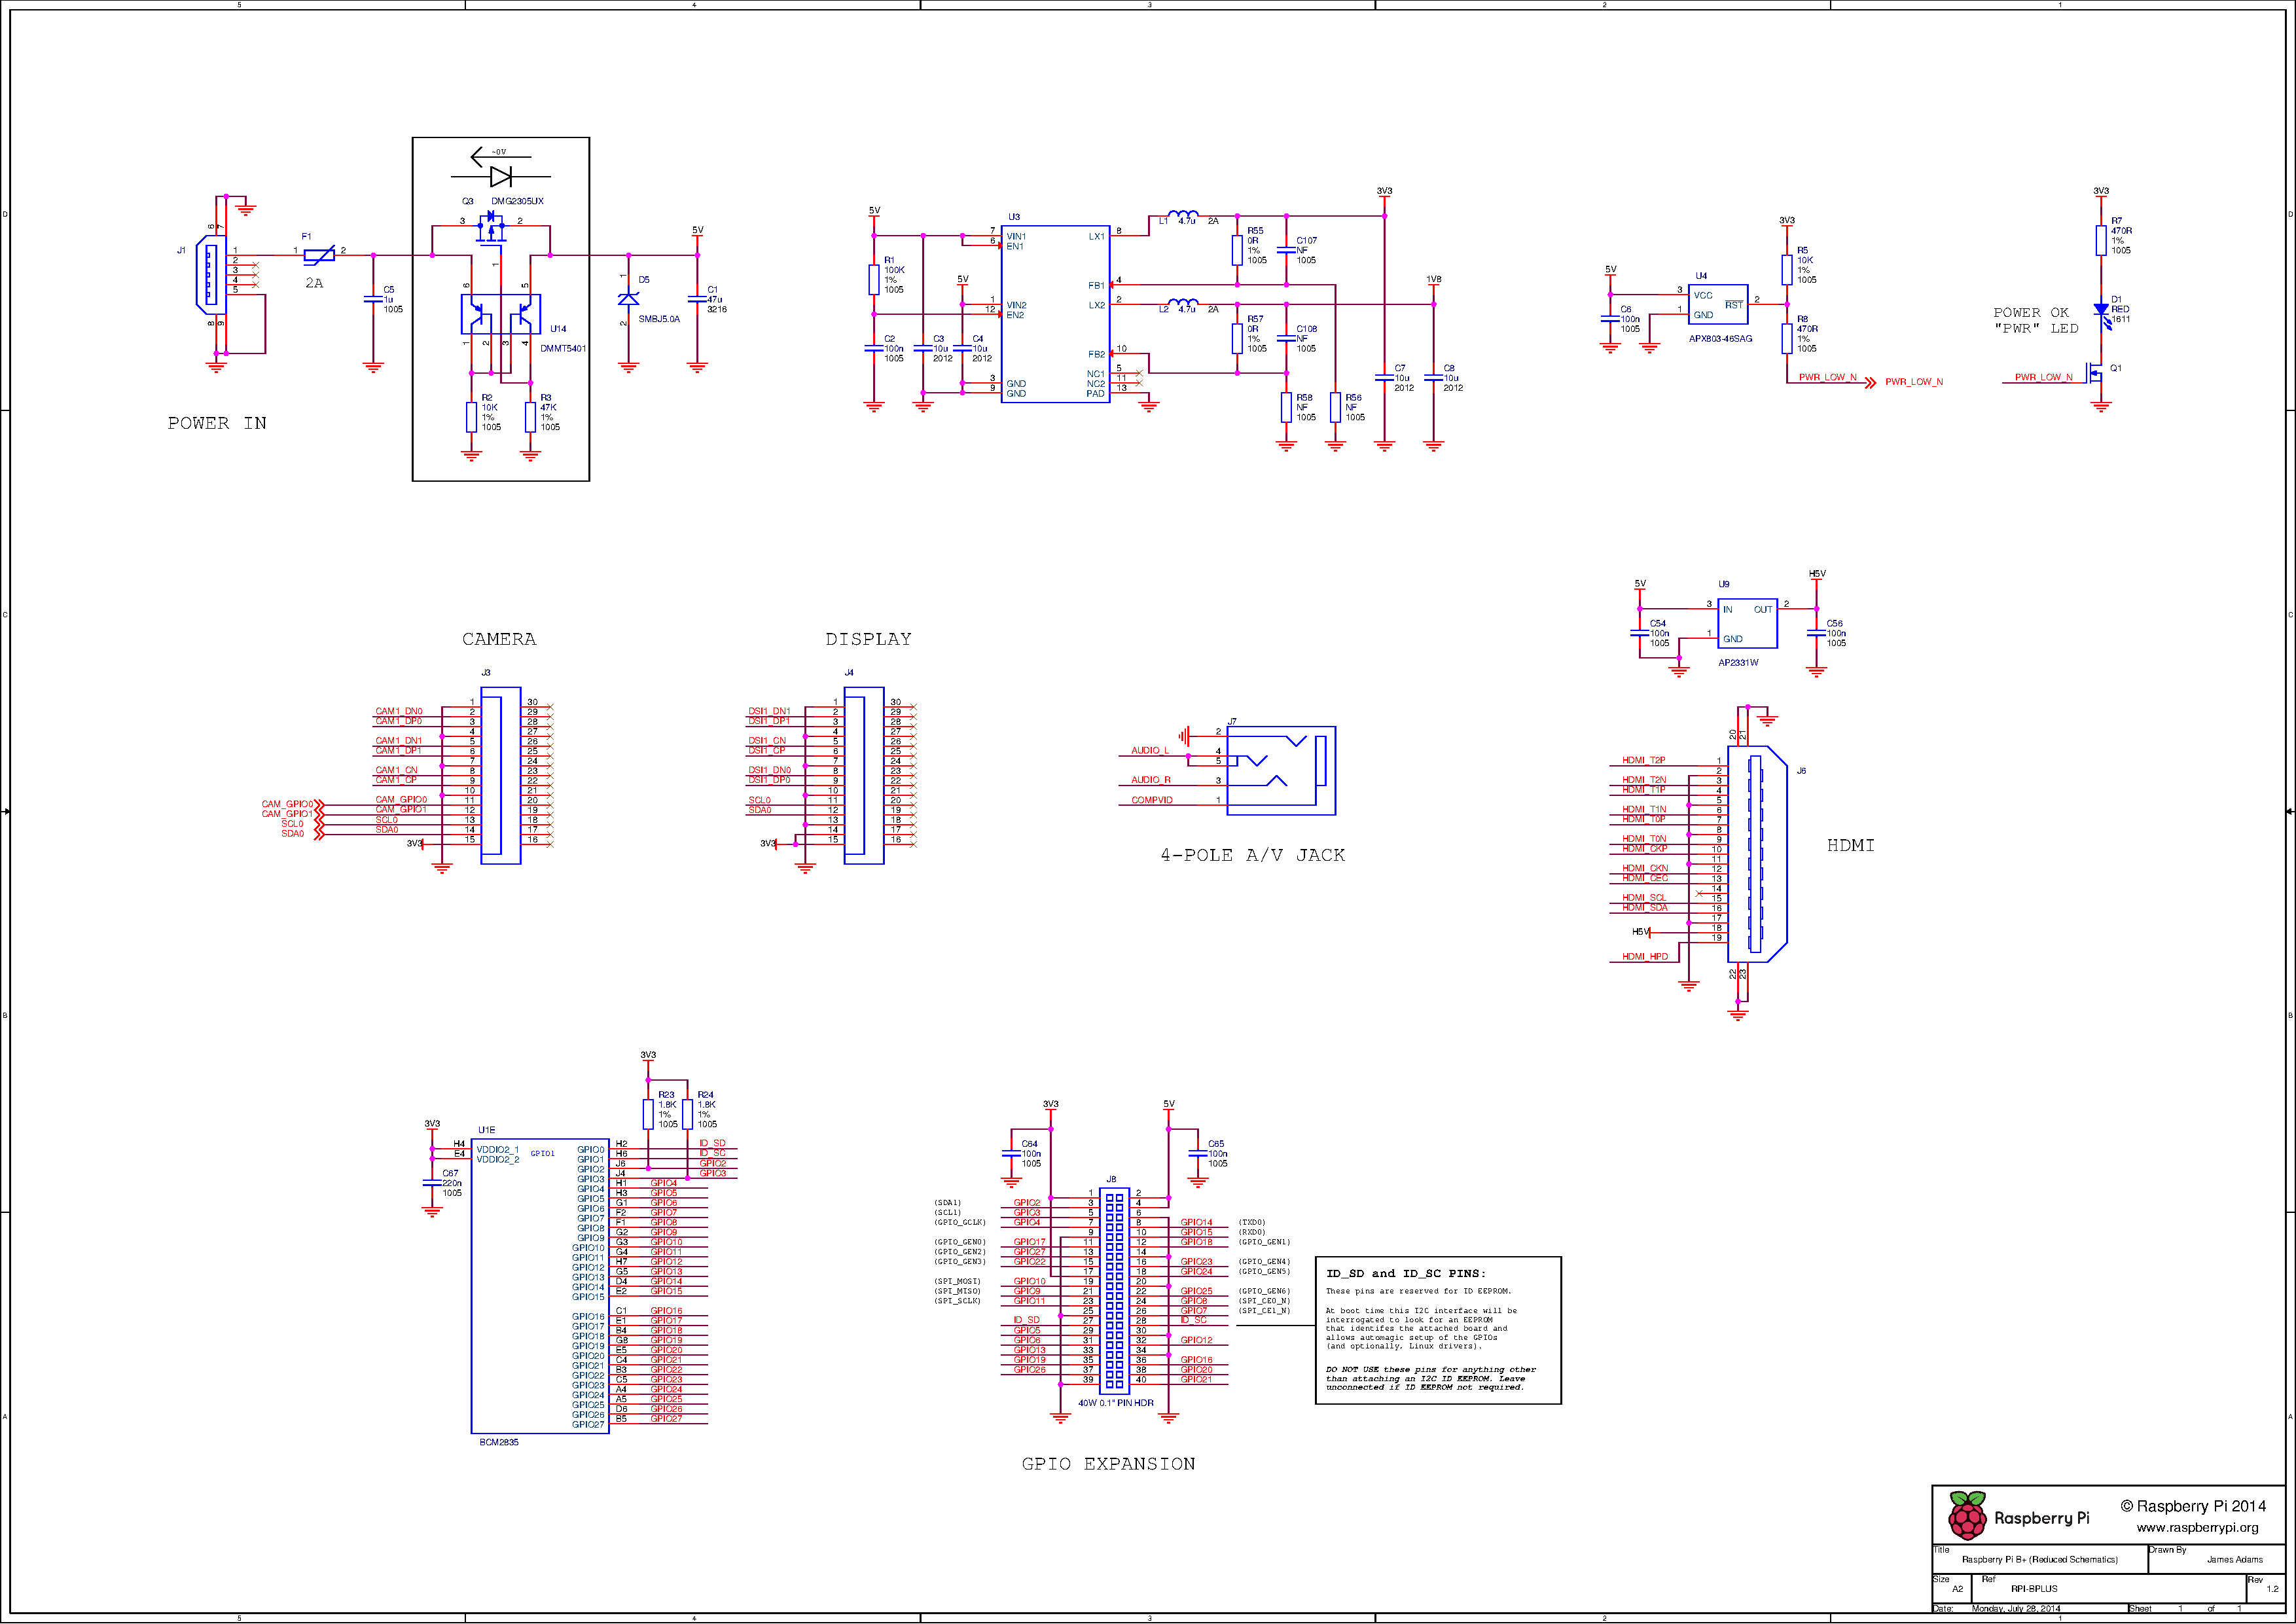
\includegraphics[width=\textwidth]{raspberrypi_doc_schema}
  \caption{Schéma technique}
\end{figure}

%%% Local Variables: 
%%% mode: latex
%%% TeX-master: "../rapport"
%%% End: 
